\chapter{Layer-dependent Activity in V1 during Stereopsis}
\ifpdf
    \graphicspath{{chapter5/chapter5-figs/PNG/}{chapter5/chapter5-figs/PDF/}{chapter5/chapter5-figs/}}
\else
    \graphicspath{{chapter5/chapter5-figs/EPS/}{chapter5/chapter5-figs/}}
\fi

\renewcommand{\runningTitle}{Layer-dependent fMRI and stereopsis}
\markboth{\MakeUppercase{\thechapter. \runningTitle }}{\thechapter. \runningTitle}

% TO DO
% - [  ] replace panels C,D in Fig 6 - need the error bars in there.
% - [  ] add stats
% - [  ] replace extrastriate by LO?

\section{Introduction}

The positional difference between the images captured by the left and right eyes, known as binocular disparity, is a highly informative cue to depth perception \cite{Wheatstone:1838xf,BLTJ:BLTJ3954}. The process of estimating depth from binocular disparity (i.e. stereopsis) is a complex process that requires multiple computational steps \cite{Marr:1976dq}. Many different cortical areas have been implicated in stereopsis \cite{Orban:2006kn,Parker:2007nx}, but their precise roles remain unclear.

Disparity processing is thought to begin in primary visual cortex, where many disparity selective neurons have been found \cite{Barlow:1967bs,Nikara:1968ys,Pettigrew:1968zr,Poggio:1977ys}. Importantly, simple subunit models are able to explain disparity selectivity in V1 relatively well, and have been instrumental in building theories of early disparity processing \cite{Ohzawa:1990cq}. However, the activity of single neurons in V1 is poorly related to stereoscopic perception \cite{Cumming:1997ve, Cumming:1999zr} --- in contrast with neurons in many extrastriate areas, such as V2 \cite{Nienborg:2007ly, Clery:2015lh}, V4 \cite{Shiozaki:2012ys}, MT \cite{Krug:2011aa} and dorsomedial visual cortex \cite{Backus:2001ly,Tsao:2003lk,Preston:2008dg}. To date, there is little data to elucidate how striate and extrastriate areas interact to support stereoscopic perception.

One promising avenue towards understanding the mechanisms by which visual areas interact is characterizing neural activity at the level of cortical layers. Because different cortical layers have largely dissociable patterns of feedforward, lateral and feedback connections, mapping neural activity at different cortical layers can reveal the flow of information (e.g. top-down or bottom-up) associated with a particular stimulus or task. For instance, recordings performed with laminar probes in macaques have helped developing new theories of how early and higher visual areas support object-based attention \cite{Self:2013qe} and working memory \cite{Kerkoerle:2017aa}. To our knowledge, this technique has not been yet used to characterize the laminar profile of neural activity evoked by stereoscopic stimuli.

Invasive and localized recording techniques require \textit{a priori} specification of a limited number of sampling sites, which hinders the investigation of multiple visual areas simultaneously. This is particularly important for investigating stereopsis given the multitude of cortical areas that have been implicated \cite{Preston:2008dg}. Ultra-high field functional resonance imaging is emerging as a promising technique to investigate the role of different cortical layers over extended regions of cortex. For instance, layer-dependent fMRI has been successfully used to extract layer-dependent BOLD signals in response to illusory figures \cite{Kok:2016fk} or partially occluded scenes \cite{Muckli:2015wb}.
% (maybe add a few more papers to the previous paragraph to strengthen the point 

Here, I set out to test the feasibility of using ultra-high field imaging at submillimetre resolution to investigate layer-dependent BOLD signals associated with stereoscopic perception. I compared the response to correlated random-dot stereograms, which elicit perception of a surface in depth, and contrast this against responses to anticorrelated random-dot stereograms, for which a surface in depth could not be perceived. I found that BOLD signals in extrastriate cortex were a strong correlate of stereoscopic perception. Conversely, little differential BOLD signals were observed in V1. Layer-dependent sampling revealed a bias towards superficial layers in LO, while an effect of cortical depth was not consistently observed in V1. Our results suggest that cortical layers in V1 and LO are differentially recruited during stereoscopic viewing and --- more generally --- that ultra-high field imaging at submillimetre resolution is a promising technique to investigate the role of different cortical layers in stereopsis.


\section{Materials and Methods}

\subsection{Participants}
Eight subjects aged between 25 and 40 years (five male) participated in the study. Participants provided informed consent and procedures were approved by the Ethics Committee of the Faculty of Psychology and Neuroscience at Maastricht University. All participants had normal or corrected-to-normal vision and did not present stereo deficits.

\subsection{Stimuli and design}
Stimuli were presented using a fiber optics goggle system (Silent Vision SV-7021, Avotec, Inc., Stuart, FL). The resulting visual field was approximately \ang{30} horizontally by \ang{23} vertically, and the viewing distance was approximately 6 cm. Stimuli consisted of random-dot stereograms (\ang{12} x \ang{12}, 34 dots/deg\textsuperscript{2}) with a mid-gray background. To promote stable vergence, the stimuli were surrounded by a static grid of squares. Dots in the stereogram followed a black or white Gaussian luminance profile, subtending \ang{0.07} at half maximum. In the center of the stereogram, four wedges were equally distributed around a circular aperture (\ang{1.2}), each subtending \ang{10} in the radial direction and \ang{70} in polar angle, with a \ang{20} gap between wedges. The wedges were presented in correlated or anticorrelated forms and had crossed or uncrossed disparity (10 arcmin, $\pm$ 0.5 arcmin jitter). The surrounding was always presented in correlated form at zero disparity. At a given time point, all wedges were rendered with the same disparity and binocular correlation. To reduce adaptation, I applied a random polar rotation to the set of wedges such that the disparity edges of the stimuli were in different locations for each stimulus presentation. In the center of the wedge field, I presented a fixation square (side length =  \ang{1}) paired with horizontal and vertical nonius lines.
Stereo correspondence and disparity sign were held constant during 12 second blocks, during which I presented 10 stimuli (900 ms on, ISI 300 ms). During each acquisition run, I presented each combination of correspondence and disparity sign 10 times, resulting in 40 blocks. In addition, there was a fixation block at the start and the end of each run. Each run lasted 504 seconds (42 blocks x 12 s), and I collected six to seven runs in each imaging session. On each run, I asked participants to fixate in the central fixation square while performing a Vernier detection task \cite{Preston:2008dg}.
For localizing activity to stimulus delivery and for quality control purposes, participants undertook one experimental run during which I presented radial checkerboard flickering at 8 Hz. The checkerboard was positioned in the center of the screen and subtended 12 degrees. Participants were instructed to fixate in the center of the screen passively while viewing the stimuli. The checkerboard was presented during 2 seconds, and was followed by a blank period of 14 seconds. A 16 second blank period was included at the beginning and at the end of the run.

\subsection{Imaging}
Imaging sessions were performed at the Maastricht Brain Imaging Center (Maastricht, The Netherlands). I used a 7 Tesla Siemens scanner with a 16-channel surface coil system. Motion was restricted by the use of foam padding. Anatomical volumes were acquired in the beginning of each session (3D-MPRAGE, 256 slices, FOV = 230x230 mm\textsuperscript{2}, matrix size = 384x384, 0.6 mm isotropic resolution), followed by a proton-density weighted volume with the same resolution and matrix size, which I used for inhomogeneity correction. I then acquired blood oxygen level-dependent (BOLD) signals during stimuli delivery. For the localizer experiment, I used two dimensional echo-planar imaging (gradient-echo; TE/TR = 24/2000 ms; flip angle = \ang{70}; FOV = 150x150 mm\textsuperscript{2}, matrix size = 136x136; 28 slices; 1.1 mm\textsuperscript{3} isotropic resolution). For the main experiment, I acquired BOLD signals using three-dimensional gradient recalled spin-echo imaging with inner volume selection (3D GRASE; TE/TR = 38/2000 ms; FOV = 24x128x9.6 mm\textsuperscript{3}, matrix size = 30x160x12, APxRLxFH; 0.8 mm\textsuperscript{3} isotropic resolution). Slice positioning was guided by visual identification of the calcarine sulcus. The acquisition volume was placed along the calcarine sulcus and efforts were made to cover both banks of the sulcus in both hemispheres, when possible.

Imaging data were analyzed using BrainVoyager QX 2.8.2 (Brain Innovation, Maastricht, The Netherlands) and custom Matlab code (The Mathworks Inc, Natick, MA). Field inhomogeneity in anatomical scans was corrected by dividing the structural volume by the respective proton-density weighted volume. When low frequency variations remained, an additional automatic inhomogeneity correction step was performed. Anatomical volumes were then manually segmented to ensure high-quality cortical representations. The resulting segmented volume was used to compute estimates of cortical thickness following the Laplace method \cite{Jones:2000cr}, from which I could later derive streamlines at different cortical depths for laminar analysis. Details on this procedure are described elsewhere \cite{Zimmermann:2011kl}. Functional data were preprocessed in functional native space to avoid unnecessary data interpolation. Head motion was estimated using trilinear interpolation and subsequently corrected using sinc interpolation. Low-frequency fluctuations were removed using a GLM with Fourier basis set at 2 cycles per run. Preprocessed data were then coregistered to the anatomical space and resampled using trilinear interpolation.

I started by defining regions of interest that were well driven by stimulus delivery. To do so, I fit a general linear model to the data, and tested for positive differences between BOLD signals during stimulus delivery and rest periods. In particular, I ensured that the region of interest comprised areas that were well modeled during the main experiment (F-contrast, stimulus versus blank, p<.005, FDR-corrected) or during the checkerboard localiser run (F-contrast, stimulus versus blank, p<0.001, FDR-corrected).
Using the cortical thickness measurements in these selected regions, I then computed nine equally spaced grids along the cortical sheet (0.1 to 0.9 in relative depth, with 0.1 increments) \cite{Zimmermann:2011kl}. Each grid intersects the cortical sheet at a different depth, and therefore runs approximately along the cortical layers. Next, the nine equally spaced grids were grouped in three equally space bins for deep, middle and superficial layers, and the corresponding cortical depth label was assigned to each voxel according to the nearest located cortical grid.

\subsection{General Linear Modeling}
For the stereo correspondence experiment, I modeled the BOLD signal using four conditions of interest (correlated, negative disparity; correlated, positive disparity; anticorrelated, negative disparity; anticorrelated, positive disparity). Advantage for stereo correlated stimuli was then tested by contrasting activity elicited by correlated versus anticorrelated blocks. These univariate procedures yield a statistic for each voxel, which one can then index by the corresponding cortical depth label assigned above.

\subsection{Multivoxel pattern analysis}
For each region-of-interest, I converted voxel time series to z-scores, and shifted the respective time course by two volumes (equivalent to four seconds) to account for the hemodynamic delay. Then, I took the median value (per voxel) across time within each condition block, resulting in 40 activity patterns per run. I trained a support vector machine classifier with leave-one-out cross-validation (i.e. leaving one run out in each fold). These resulted in 240 patterns for training and 40 patterns for testing the model (less 40 training patterns for one subject for which I acquired only six runs of the main experiment). For each cross-validation fold, I stored the absolute weights assigned to each voxel by the classifier, and examine their distribution at different cortical depths. As mentioned above, I divided voxels in three groups according to their relative distance from the white matter: deep layers (from 0.1 to 0.3); intermediate layers (relative depths from 0.4-0.6); and superficial layers (from 0.7-0.9).

\section{Results}
I recorded blood oxygenation level-dependent signals while participants fixated on a central cross and viewed correlated and anticorrelated random-dot stereograms. The stereograms consisted of four concentric wedges rendered in correlated  or anticorrelated form; in the former, the wedges were perceived in depth; in the latter, no depth perception emerged. In order to localize responsive areas, I ran an additional experiment during which a flickering checkerboard was presented to both eyes, interleaved with blank periods.

It is known that gradient-echo (GE) based sequences are considerably biased by macrovasculature, even at ultra-high field strengths \cite{DeMartino:2013qy}. Because of the high density of such large veins near the pial surface, layer-dependent BOLD signals acquired with GE sequences typically suffer of large biases towards superficial layers \cite{Polimeni:2010fl,Koopmans:2010hq}. Spin-echo based sequences, such as 3D GRASE, have proved more immune to macrovasculature contributions and thus provide increase cortical specificity \cite{DeMartino:2013qy}. I chose the 3D GRASE sequence for this reason.

However, using 3D GRASE also imposes considerable restrictions on data acquisition and analysis. First and foremost, 3D GRASE offers less sensitivity to BOLD changes when compared to GE sequences \cite{DeMartino:2013qy}. Another worrying restriction is very limited coverage --- while this is usually not an issue for conventional fMRI, the increase in resolution effectively decreases the volume of brain that can be covered by a particular number of slices. With 12 slices and a slice thickness of 0.8 mm, I was limited to covering 9.6 millimeters along the superior-inferior direction. Although the main interest was in imaging early visual areas, the extended coverage in the left-right direction effectively allowed coverage of lateral occipital areas as well (Fig. \ref{fig:ch5fig2}). Slice positioning was guided by visual identification of the calcarine sulcus. Whenever possible, the slice was angled so as to cover both banks of the calcarine sulcus while maximizing coverage of lateral extrastriate areas in both hemispheres (Fig. \ref{fig:ch5fig2}).

\begin{figure}
  \centering
  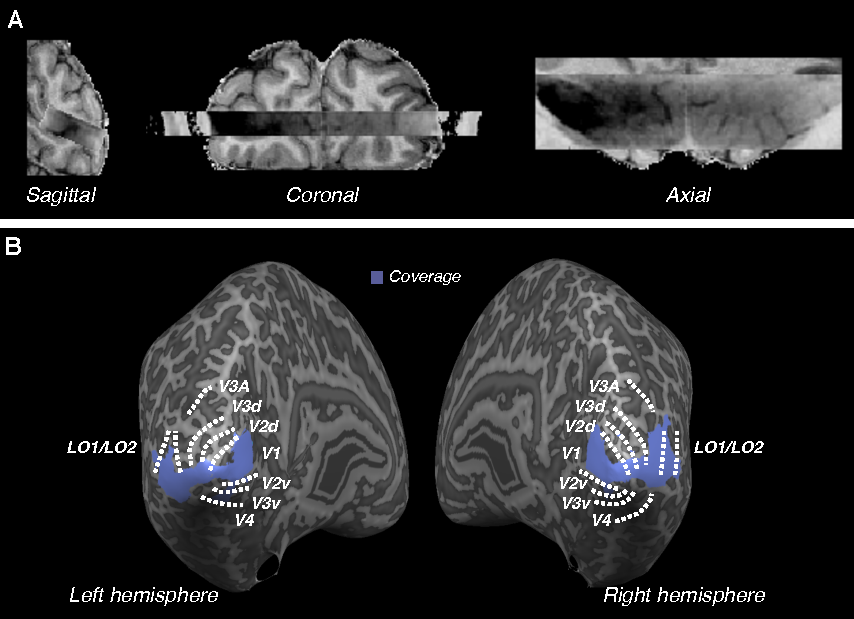
\includegraphics[keepaspectratio]{Fig2.pdf}
  \caption[Imaging field-of-view for the main experiment.]{Imaging field-of-view for the main experiment. (A) The acquisition slab was placed parallel to the calcarine sulcus, attempting to image both hemispheres equally. (B) Previously collected retinotopic maps showed that the slab covered mainly V1 and lateral occipital areas LO1 and LO2.}
  \label{fig:ch5fig2}
\end{figure}

Reduced coverage and high-resolution acquisitions also challenge off-the-shelf preprocessing tools. In particular, traditional algorithms for motion correction often fail to converge to the correct solution. I have experienced this issue for all our participants, even though they typically moved less than 1 millimeter within an entire session. To compensate for this issue, I used a coarse-to-fine, exhaustive grid-search procedure for motion correction. I started by computing the similarity (here Pearson's correlation) between the reference and source scan for all possible points on a 6-dimensional grid (3 for translation and 3 for rotation) with five elements per dimension, and with each dimension spanning between $\pm 1$ millimeter or degree. Thereafter, I chose the combination of parameters that produced the highest similarity, and then performed another iteration of grid-search over a smaller grid. This approach, although laborious, outperformed traditional algorithms for motion correction.

Despite the challenges, I obtained strong responses to stimulus delivery across striate and extrastriate areas (Fig. \ref{fig:ch5fig2}). Contrary to conventional fMRI data, our high-resolution protocol at ultra-high field yielded activity clusters that were well confined to the gray matter. Based on the F-statistic of the GLMs fit to the main experiment and to the localiser experiment, I identified two regions that were consistently driven by stimulus delivery across participants: a region of interest in the calcarine sulcus and another one in lateral occipital cortex. Retinotopy data confirmed that these two ROIs corresponded to areas V1 and LO (areas LO1/LO2), respectively.

\begin{figure}
  \centering
  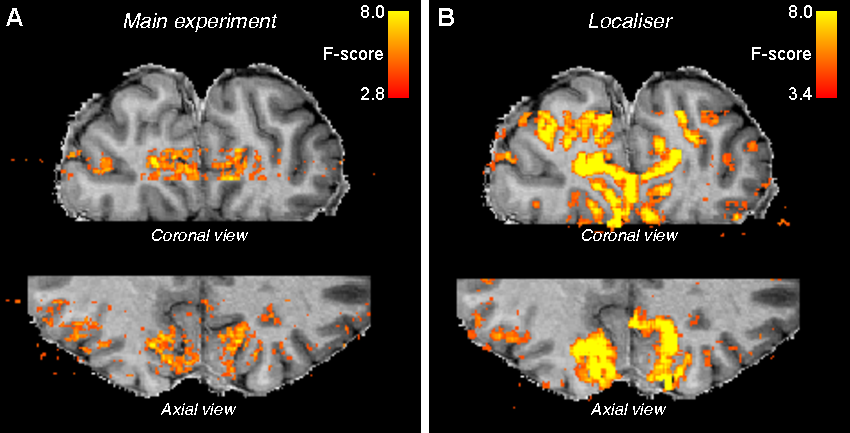
\includegraphics[keepaspectratio]{Fig3.pdf}
  \caption[General linear modeling of stimulus related activity.]{General linear modeling of task related activity demonstrated that our imaging protocol captured changes in signal associated with stimulus presentation, both in the main experiment (A) and in the localiser experiment (B).}
  \label{fig:ch5fig3}
\end{figure}

Having confirmed the suitability of our imaging protocol, I then sought to examine the distribution of BOLD signal change across different cortical layers. To do so, I generated cortical grid meshes at different relative cortical depths between the white-matter/gray-matter boundary and the pial (Fig. \ref{fig:ch5fig4}A). This allowed me to assign a cortical depth label to each voxel within a region of interest. I did this via nearest-neighbour interpolation---that is, a particular voxel was assigned the relative cortical depth label corresponding the that of the closest cortical grid mesh. I then divided the cortical depth labels in three bins --- deep, middle and superficial layers --- and finally looked at the difference between activity evoked by correlated and anticorrelated RDS. In early visual cortex, I found little activity and no evident differences across layers (Fig. \ref{fig:ch5fig4}B). In contrast, I found a much greater effect in extrastriate areas, where a bias towards superficial layers was also evident. Thus, on the basis of univariate signals, I found a preference for stereopsis in lateral occipital cortex, but not in early visual cortex.

\begin{figure}
  \centering
  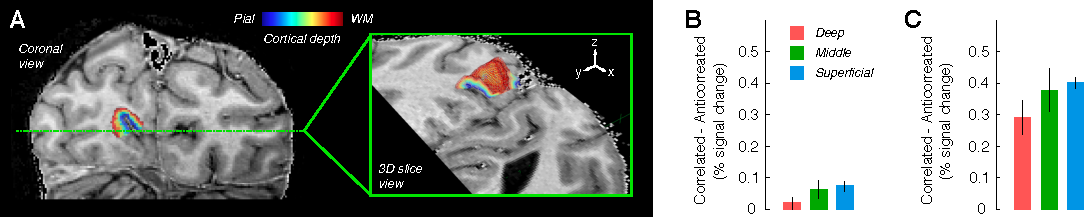
\includegraphics[keepaspectratio,width=14cm]{Fig4.pdf}
  \caption[Layer-dependent activity in striate and extrastriate cortex.]{Layer-dependent activity in striate and extrastriate cortex (A). The Laplace layer sampling method \cite{Jones:2000cr} was used to obtain a cortical depth label for each voxel within the V1 and LO regions of interest. I found little difference in univariate V1 signal for correlated and anticorrelated stimuli (B). Conversely, I observed greater overall activation in LO relative to V1, and an apparent increase in layer-dependent activity towards superficial layers. Error bars denote standard error across participants.}
  \label{fig:ch5fig4}
\end{figure}

Based on our previous analysis, concluding that activity in primary visual cortex was not related to stereoscopic perception would be premature. In particular, it is possible that fMRI measurements in V1 encapsulate stimulus related information across the activity of multiple instead of single voxels. To examine this possibility, I used support vector machines to decode binocular stimulus correlation (cRDS \textit{vs.} aRDS) based on the pattern of activity across a population of voxels. Using a searchlight approach, I found that it was indeed possible to decode the stimulus class above chance level in both primary visual and lateral occipital cortex (Fig. \ref{fig:ch5fig5}).

\begin{figure}
  \centering
  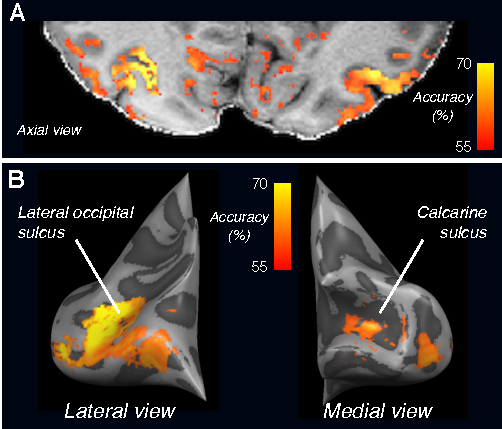
\includegraphics[keepaspectratio]{Fig5.pdf}
  \caption[Searchlight classification for cRDS vs aRDS.]{Searchlight classification for cRDS \textit{vs} aRDS for a representative subject in volume (A) and cortical surface (B) space. I found above chance accuracy in primary visual cortex as well as lateral occipital areas.}
  \label{fig:ch5fig5}
\end{figure}

Having established that both V1 and lateral occipital contain multivariate signals related to our experimental manipulation, I then asked whether such signals depend on cortical depth. To do so, I used the cortical depth sampling labels (see above) to subdivide voxels in three sub-ROIs: deep, middle and superficial layers. Consistent with our previous univariate analysis, I found a higher decoding accuracy in extrastriate relative to primary visual cortex and an apparent bias towards superficial layers (Fig. \ref{fig:ch5fig6}A,B; compare with Fig. \ref{fig:ch5fig4}B,C).

One possible concern with our previous approach is that binning voxels into `deep', `middle' and `superficial' layers is somewhat arbitrary, and often biases the number of features (i.e. voxels) available for multivariate analysis (e.g. in the fundus of a sulcus one may observe that more voxels are assigned to deep relative to superficial layers). Therefore, instead of subdividing each ROI in different layers, I trained classifiers using the entire pattern of voxels in an ROI, and then examined the weights attributed to voxels as a function of cortical depth. I found that the classifier assigned systematically higher weights to the superficial layers in lateral occipital areas (Fig. \ref{fig:ch5fig6}D), but that pattern was not observed for V1 (Fig. \ref{fig:ch5fig6}C).

\begin{figure}
  \centering
  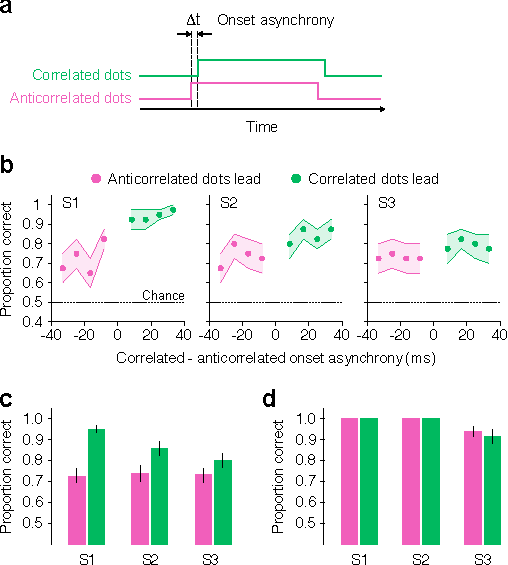
\includegraphics[keepaspectratio]{Fig6}
  \caption[ROI based multivariate classification analysis.]{ROI based multivariate classification analysis. Classification accuracy (A, B) and classifier weights (C, D) per layer in V1 (A, C) and LO (B, D). These results indicate a bias towards superficial layers in LO, but not in V1. Error bars depict standard error across participants.}
  \label{fig:ch5fig6}
\end{figure}


\section{Discussion}

Here, I have examined how human visual cortex responds in the presence and absence of stable three-dimensional perception as measured using sub-millimeter fMRI. I manipulated perceptual relevance by using correlated and anticorrelated random-dot stereograms. Correlated stereograms could be easily fused to perceive a three-dimensional surface, while anticorrelated stimuli could not, and therefore did not elicit stable three-dimensional perception. Using ultra-high field imaging with isotropic sub-millimeter resolution, I investigated BOLD responses to these stimuli at different cortical layers of primary and lateral-occipital visual cortex. I observed evident univariate signal change in LO during periods of stable three-dimensional perception, while less differential signals were found in primary visual cortex. Multivariate pattern classification analyses confirmed this dissociation between V1 and LO. Most importantly, our results suggest that ultra-high field fMRI is a valuable tool to examine layer-dependent activity associated with stereopsis.


\subsection{Methodological limitations and neurovascular origin}

Given that BOLD measurements are a haemodynamic proxy of neural activity, the right interpretation of our experimental results must also be a cautious one. I acquired BOLD signals at sub-millimeter resolution to investigate responses of neural populations in different cortical layers. Although the BOLD signal appears to be more locally registered to neural activity than previously thought \cite{Siero:2014it}, it is reasonable to assume that biases in the type and amount of vasculature across the cortical layers \cite{Duvernoy:1981yq} may influence our results.

I have incorporated several measures to avoid vascular biases from interfering with the results. In particular, by scanning at ultra-high field, I greatly reduce macrovascular contributions \cite{Gati:1997uq,Ogawa:1998fk,Ugurbil:2003uq}. Additionally, I chose to use a spin-echo based sequence (3D GRASE \cite{Feinberg:2008qa}) to provide increased spatial specificity --- this sequence has an estimated point-spread function of approximately 0.5 mm (Gaussian FWHM) and is more immune to macrovascular contributions \cite{DeMartino:2013qy}. These characteristics of our imaging protocol are likely to have largely attenuated, if not eliminated, the large macrovascular biases that typically corrupt the BOLD signal.

To our knowledge, our study was the first attempt to examine how different cortical layers are involved in human stereoscopic perception. As I highlighted earlier, such endeavour posed significant challenges at the level of data acquisition and analysis. On the analysis side, reduced coverage and high-resolution data required the development of new preprocessing and analysis pipelines for fMRI data --- some of which will keep improving as the community develops new tools and converges to best practices. For instance, methods for more accurate cortical depth sampling are being developed and are likely to become standard in the near future \cite{Waehnert:2013kl}.

On the data acquisition end, I faced stringent limits on coverage. I followed a quality by design approach by choosing 3D GRASE over a gradient-echo based sequence, since this provided the least opportunity for observing macrovascular driven effects \cite{DeMartino:2013qy}. Unfortunately, this entailed working with reduced coverage and lower signal-to-noise ratio. Future work might choose follow a quality by control approach instead. Using a gradient-echo based sequence will provide room for increasing coverage and will also yield higher signal-to-noise ratio: the former would allow to simultaneously image many of the areas involved in stereopsis (potentially even the whole brain via multiband imaging); the latter would increase the likelihood of detecting small effects or potentially reduce the duration of each experiment, which effectively attenuates the impact of head motion. The main drawback would then relate to the interpretability of cortical profiles --- the true pattern of layer-dependent activation might be masked by a mixture of signals poorly related to local neural activity. Finally, cerebral blood volume (CBV) measurements are also a promising technique that could be used for probing layer-dependent activity in the cortex. It has been shown that CBV measurements provide increase specificity and are therefore more interpretable than gradient-echo BOLD measurements \cite{Huber:2015ao}. However, as with 3D GRASE, CBV measurements impose tighter constraints on coverage.

An important pathway to establish the best protocol for imaging would be to validate layer-dependent fMRI measurements against observations made by neuroanatomists and neurophysiologists. A simple benchmark exists in the case of stereopsis: I know from a vast body of physiological work that neurons in layer 4C in V1 are monocular, and that binocularity increases towards supra- and infragranular layers. Therefore, I would expect little or no binocular information around intermediate cortical layers, and substantial binocular information in superficial and deep layers. However, that was not what I observed. Although I prioritized spatial specificity in choosing 3D GRASE, it is possible that the degree of specificity of the sequence is not high enough to detect such a U-shaped cortical profile --- particularly if voxels in intermediate layers are contaminated by activity from supragranular and infragranular layers.


\subsection{The role of cortical layers in stereoscopic vision}

Our results suggest that activity in superficial layers of lateral occipital regions is a better correlate of stable stereoscopic perception than that of early visual areas (Figs. \ref{fig:ch5fig4} and \ref{fig:ch5fig6}). While this is a novel and interesting finding, an explanatory account of the involvement of superficial layers of LO in stereoscopic processing cannot be built based on our data alone (or based on any fMRI dataset in general). However, I do find evidence for different profiles of activation across layers in primary visual and lateral occipital cortex. In what follows, I venture some potential explanations for our observations.

One possibility is that individual neurons in superficial layers of lateral occipital cortex are not selective for disparity in anticorrelated RDS. Neurophysiological investigations suggest that the response to anticorrelated stimuli decreases as we go up the cortical hierarchy \cite{Cumming:1997ve,Tanabe:2004mw}, and eventually disappears in areas of the visual cortex specialized for object recognition \cite{Janssen:2003fk}. Therefore, the preference for stereopsis that I observe in superficial layers of lateral occipital cortex could be a reflection of this feedforward process, which typically propagates through superficial layers of cortex.

Another possibility is that the nature of coding of stereoscopic information differs between primary visual and lateral occipital cortex. It is possible that stereoscopic information in primary visual cortex is dispersed across layers and is multivariate in nature. There is at least evidence against a univariate code because many individual V1 neurons have opposite disparity tuning curves for correlated and anticorrelated RDS \cite{Cumming:1997ve}. On the other hand, neural activity at the level of individual neurons in LO might be more informative about stereo correspondence. Thus, it is possible that the differences in the laminar profile between V1 and LO reflect distinct coding principles rather than absence or presence of signals that support stereopsis.

Finally, it is also possible that the differences between the laminar profiles observed in V1 and LO are a consequence of the underlying cortical organization. In V1, it is known that neurons with different selectivity for binocular disparity are typically intermixed \cite{Prince:2002cr}, and this lack of clustering could limit the detection of disparity selective responses as measured with fMRI. Conversely, as shown in the previous chapter, clustering for binocular disparity has been observed across many extrastriate areas, including area V3B/KO --- an area located just next to LO. Thus, it is possible that an increase in clustering of disparity selective neurons in LO facilitated the detection of layer-dependent changes in this area, while the lack of clustering hindered the detection of a similar effect in V1.



% ------------------------------------------------------------------------

%%% Local Variables: 
%%% mode: latex
%%% TeX-master: "../thesis"
%%% End: 
